\documentclass{article}
\usepackage[utf8]{inputenc}
\usepackage{listings}
\usepackage{graphicx}
\usepackage{float}
\usepackage{xcolor}
\usepackage{geometry}
\usepackage{CJKutf8}
\usepackage{amsmath}
\usepackage{amssymb}

\geometry{a4paper,scale=0.8}
\lstset{
    basicstyle          =   \sffamily,        
    keywordstyle        =   \bfseries,         
    commentstyle        =   \rmfamily\itshape, 
    stringstyle         =   \ttfamily, 
    flexiblecolumns,               
    numbers             =   left,  
    showspaces          =   false, 
    showstringspaces    =   false,
    captionpos          =   t,     
    frame               =   lrtb, 
}

\lstdefinestyle{Python}{
    language        =   Python, % 语言选Python
    basicstyle      =   \zihao{-5}\ttfamily,
    numberstyle     =   \zihao{-5}\ttfamily,
    keywordstyle    =   \color{blue},
    keywordstyle    =   [2] \color{teal},
    stringstyle     =   \color{magenta},
    commentstyle    =   \color{red}\ttfamily,
    breaklines      =   true,  
    columns         =   fixed,  
    basewidth       =   0.5em,
}

\title{\bf\Large  概率论与数理统计 第7次作业}
%%%%%%%%%%%%%%%%%%%%%%%%%%%%%%%%%%%%%%
%% DON'T forget to change this part %%
\author{\bf Name: 宋昊原 \qquad Student ID: 2022010755}
%%%%%%%%%%%%%%%%%%%%%%%%%%%%%%%%%%%%%%

\begin{document}
\begin{CJK}{UTF8}{gbsn}
\maketitle
\section{二项分布}
\subsection{概率密度函数图}
\begin{minipage}{0.5\textwidth}
    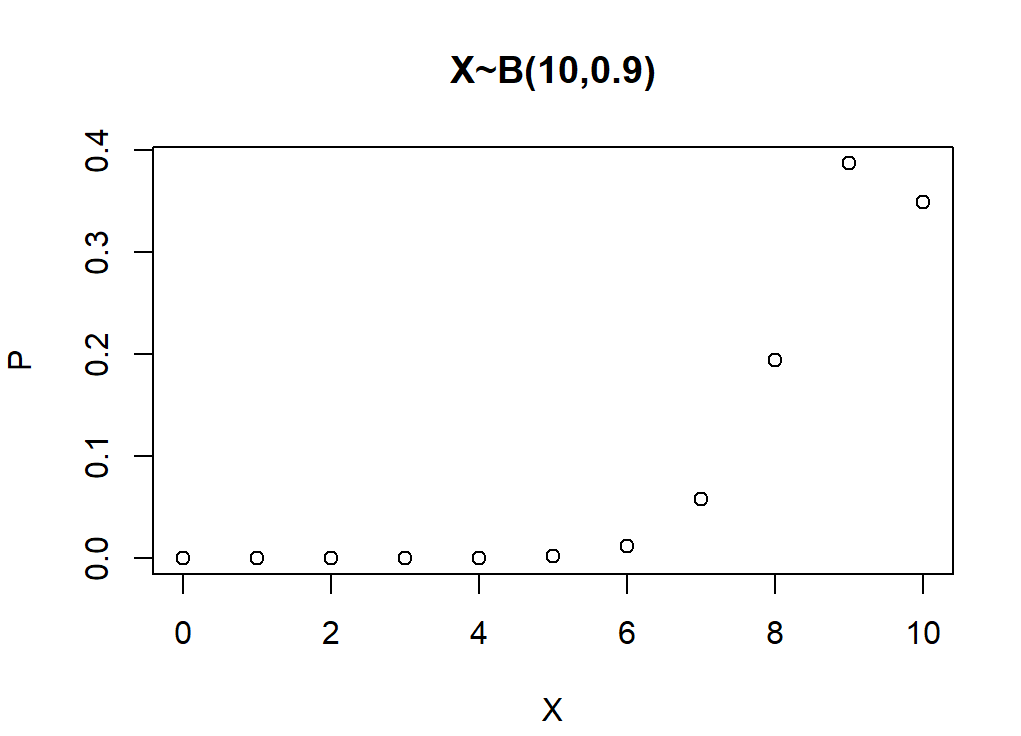
\includegraphics[scale=0.6]{plot1X.png}
\end{minipage}
\\
\begin{minipage}{0.5\textwidth}
    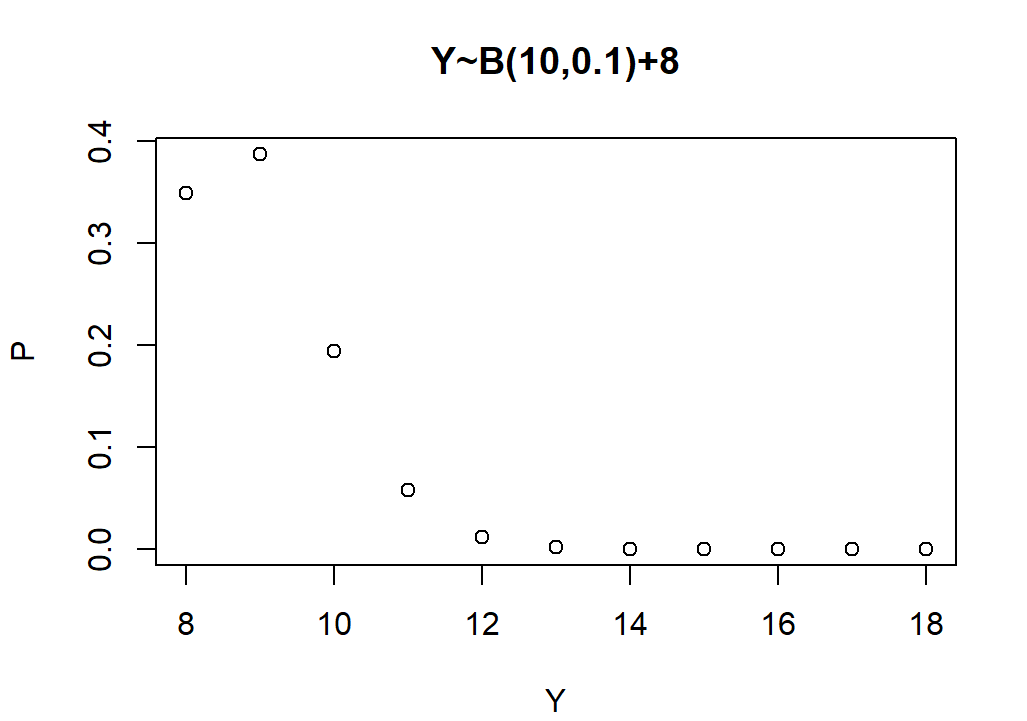
\includegraphics[scale=0.6]{plot1Y.png}
\end{minipage}
\subsection{均值、方差、中位数、众数}
均值:\\
$$ X:9,Y:9 $$
方差:\\
$$ X:0.9,Y:0.9 $$
中位数:\\
$$ X:9,Y:9 $$
众数:\\
$$ X:9,Y:9 $$
\subsection{偏度系数}
$$ Skew(X)=-0.988,\ Skew(Y)=0.988 $$
\section{各种分布的矩}
设$X\sim Exp(1),\ Y\sim P(4),\ Z\sim U(0,1)$.
\subsection{}
$$ E(X)=1,\ Var(X)=1 $$
$$ Skew(X)=E((X-1)^{3})=\int_{0}^{+\infty}(x-1)^{3}e^{-x}dx=-\int_{0}^{+\infty}(x-1)^{3}d(e^{-x})$$
$$ =-(x-1)^{3}e^{-x}|_{0}^{+\infty}+3\int_{0}^{+\infty}(x-1)^{2}e^{-x}dx $$
$$ =-1+3Var(X)=2$$
$$ Kurt(X)=E((X-1)^{4})=\int_{0}^{+\infty}(x-1)^{4}e^{-x}dx=-\int_{0}^{+\infty}(x-1)^{4}d(e^{-x})$$
$$ =-(x-1)^{4}e^{-x}|_{0}^{+\infty}+4\int_{0}^{+\infty}(x-1)^{3}e^{-x}dx$$
$$ =1+4Skew(X)=9$$
\\\\
$$ E(Y)=4,\ Var(Y)=4 $$
$$ Skew(Y)=\frac{1}{8}E((Y-4)^{3})=\frac{1}{8}\sum\limits_{k=0}^{+\infty}(k-4)^{3}\frac{4^{k}e^{-4}}{k!}$$
$$ =\frac{1}{2}\sum\limits_{k=1}^{+\infty}(k-4)^{2}\frac{4^{k-1}e^{-4}}{(k-1)!}-\frac{1}{2}\sum\limits_{k=0}^{+\infty}(k-4)^{2}\frac{4^{k}e^{-4}}{k!}$$
$$ =\frac{1}{2}\sum\limits_{k=0}^{+\infty}(k-3)^{2}\frac{4^{k}e^{-4}}{k!}-\frac{1}{2}Var(Y)$$
$$ =\frac{1}{2}\sum\limits_{k=0}^{+\infty}(k-4)^{2}\frac{4^{k}e^{-4}}{k!}+4\sum\limits_{k=1}^{+\infty}\frac{4^{k-1}e^{-4}}{(k-1)!}-\frac{7}{2}\sum\limits_{0}^{+\infty}\frac{4^{k}e^{-4}}{k!}-\frac{1}{2}Var(Y)$$
$$ =\frac{1}{2}Var(Y)+4\times 1-\frac{7}{2}\times 1-\frac{1}{2}Var(Y)=\frac{1}{2}$$
$$ Kurt(Y)=\frac{1}{16}E((Y-4)^{4})=\frac{1}{16}\sum\limits_{k=0}^{+\infty}(k-4)^{4}\frac{4^{k}e^{-4}}{k!}$$
$$ =\frac{1}{4}\sum\limits_{k=1}^{+\infty}(k-4)^{3}\frac{4^{k-1}e^{-4}}{(k-1)!}-\frac{1}{4}\sum\limits_{k=0}^{+\infty}(k-4)^{3}\frac{4^{k}e^{-4}}{k!}$$
$$ =\frac{1}{4}\sum\limits_{k=0}^{+\infty}(k-3)^{3}\frac{4^{k}e^{-4}}{k!}-2Skew(Y)$$
$$ =\frac{1}{4}\sum\limits_{k=0}^{+\infty}((k-4)^{3}+3(k-4)^{2}+3(k-4)+1)\frac{4^{k}e^{-4}}{k!}-2Skew(Y)$$
$$ =2Skew(Y)+\frac{3}{4}Var(Y)+0+1-2Skew(Y)=\frac{13}{4}$$
\\\\
$$ E(Z)=\frac{1}{2},\ Var(Y)=\frac{1}{12} $$
$$ Skew(Y)=24\sqrt{3}E((Z-\frac{1}{2})^{3})=24\sqrt{3}\int_{0}^{1}(z-\frac{1}{2})^{3}dz$$
$$ =24\sqrt{3}\int_{0}^{1}(z^{3}-\frac{3}{2}z^{2}+\frac{3}{4}z-\frac{1}{8})dz$$
$$ =24\sqrt{3}(\frac{1}{4}-\frac{1}{2}+\frac{3}{8}-\frac{1}{8})=0$$
$$ Kurt(Y)=144E((Z-\frac{1}{2})^{4})=144\int_{0}^{1}(z-\frac{1}{2})^{4}dz$$
$$ =144\int_{0}^{1}(z^{4}-2z^{3}+\frac{3}{2}z^{2}-\frac{1}{2}z+\frac{1}{16})dz$$
$$ =144(\frac{1}{5}-\frac{1}{2}+\frac{1}{2}-\frac{1}{4}+\frac{1}{16})$$
$$ =\frac{9}{5}$$
\subsection{}
$$ M_{X}(t)=E(e^{tX})=\int_{0}^{+\infty}e^{xt}e^{-x}dx$$
$$ =\int_{0}^{+\infty}e^{(t-1)x}dx=\frac{1}{t-1}\int_{0}^{+\infty}e^{(t-1)x}d((t-1)x)$$
$$ =\frac{1}{1-t},\ t<1$$
\\\\
$$ M_{Y}(t)=E(e^{tY})=\sum\limits_{k=0}^{+\infty}e^{kt}\frac{4^{k}e^{-4}}{k!}$$
$$ =\frac{1}{e^{4}}\sum\limits_{k=0}^{+\infty}\frac{(4e^{t})^{k}}{k!}=e^{4(e^{t}-1)}$$
\\\\
$$ M_{Z}(t)=E(e^{tZ})=\int_{0}^{1}e^{zt}dz=\frac{e^{t}-1}{t}$$
特别地,$M_{Z}(0)=1$.
\subsection{}
$$ M_{X}'(t)=\frac{1}{(1-t)^{2}}\Rightarrow E(X)=M_{X}'(0)=1 $$
$$ M_{X}^{(2)}(t)=\frac{2}{(1-t)^{3}}\Rightarrow E(X^{2})=M_{X}^{(2)}(0)=2 $$
$$ M_{X}^{(3)}(t)=\frac{6}{(1-t)^{4}}\Rightarrow E(X^{3})=M_{X}^{(3)}(0)=6 $$
$$ M_{X}^{(4)}(t)=\frac{24}{(1-t)^{5}}\Rightarrow E(X^{4})=M_{X}^{(4)}(0)=24 $$
故
$$ Skew(X)=E((X-1)^{3})=E(X^{3})-3E(X^{2})+3E(X)-1=2$$
$$ Kurt(X)=E((X-1)^{4})=E(X^{4})-4E(X^{3})+6E(X^{2})-4E(X)+1=9$$
\\\\
$$ M_{Y}'(t)=4e^{t}e^{4(e^{t}-1)}\Rightarrow E(X)=M_{Y}'(0)=4$$
$$ M_{Y}^{(2)}(t)=(4e^{t}+16e^{2t})e^{4(e^{t}-1)}\Rightarrow E(X^{2})=M_{Y}^{(2)}(0)=20$$
$$ M_{Y}^{(3)}(t)=(4e^{t}+48e^{2t}+64e^{3t})e^{4(e^{t}-1)}\Rightarrow E(X^{3})=M_{Y}^{(3)}(0)=116$$
$$ M_{Y}^{(4)}(t)=(4e^{t}+112e^{2t}+384e^{3t}+256e^{4t})e^{4(e^{t}-1)}\Rightarrow E(X^{4})=M_{Y}^{(4)}(0)=756$$
故
$$ E((Y-4)^{3})=E(Y^{3})-12E(Y^{2})+48E(Y)-64=4$$
$$ Skew(Y)=\frac{1}{8}E((Y-4)^{3})=\frac{1}{2}$$
$$ E((Y-4)^{4})=E(Y^{4})-16E(Y^{3})+96E(Y^{2})-256E(Y)+256=52$$
$$ Kurt(Y)=\frac{1}{16}E((Y-4)^{4})=\frac{13}{4}$$
\\\\
$$ M_{Z}(t)=\frac{e^{t}-1}{t}=\frac{\sum\limits_{n=1}^{+\infty}\frac{t^{n}}{n!}}{t}=\sum\limits_{n=0}^{+\infty}\frac{t^{n}}{(n+1)!}$$
于是
$$ E(X^{k})=M_{Z}^{(k)}(0)=\frac{k!}{(k+1)!}=\frac{1}{k+1}$$
故
$$ Skew(Z)=24\sqrt{3}E((X-\frac{1}{2})^{3})=24\sqrt{3}(E(X^{3})-\frac{3}{2}E(X^{2})+\frac{3}{4}E(X)-\frac{1}{8})$$
$$ =24\sqrt{3}(\frac{1}{4}-\frac{1}{2}+\frac{3}{8}-\frac{1}{8})=0$$
$$ Kurt(Z)=144E((X-\frac{1}{2})^{4})=144(E(X^{4})-2E(X^{3})+\frac{3}{2}E(X^{2})-\frac{1}{2}E(X)+\frac{1}{16})$$
$$ =144(\frac{1}{5}-\frac{1}{2}+\frac{1}{2}-\frac{1}{4}+\frac{1}{16})=\frac{9}{5}$$
\section{由矩母函数求分布}
首先考虑指数分布$Y\sim Exp(\lambda)$的矩母函数.
$$ M_{Y}(t)=E(e^{tY})=\int_{0}^{+\infty}\lambda e^{(t-\lambda)y}dy=\frac{\lambda}{\lambda-t}$$
令$Y_{2}\sim Exp(2),\ Y_{3}\sim Exp(3)$,则
$$ M_{X}(t)=\frac{1}{3}M_{Y_{2}}(t)+\frac{2}{3}M_{Y_{3}}(t)$$
故
$$ f_{X}(x)=\frac{1}{3}f_{Y_{2}}(x)+\frac{2}{3}f_{Y_{3}}(x)=\frac{2}{3}e^{-2x}+2e^{-3x},\ x>0$$
\section{对数正态分布}
\subsection{}
$$ E(e^{tY})=E(e^{te^{X}})=\frac{1}{\sqrt{2\pi}\sigma}\int_{-\infty}^{+\infty}\exp(-\frac{(x-\mu)^{2}}{2\sigma^{2}}+te^{x})dx$$
被积函数在$x$趋于某一侧无穷时极限为$+\infty$,故积分不存在.
\subsection{}
$$ M_{X}(t)=e^{\mu t+\frac{(\sigma t)^{2}}{2}}$$
而
$$ E(Y^{n})=E(e^{nX})=M_{X}(n)=e^{\mu n+\frac{(\sigma n)^{2}}{2}}$$
\section{独立Poisson分布的和}
考虑$X_{i}$的矩母函数
$$ M_{X_{i}}(t)=E(e^{tX_{i}})=\sum\limits_{k=0}^{\infty}e^{kt}\frac{\lambda_{i}^{k}e^{-\lambda_{i}}}{k!}=e^{-\lambda_{i}}\sum\limits_{k=0}^{\infty}\frac{(\lambda_{i} e^{t})^{k}}{k!}=e^{\lambda_{i}(e^{t}-1)}$$
则
$$ M_{Y}(t)=M_{X_{1}}(t)M_{X_{2}}(t)=e^{\lambda_{1}(e^{t}-1)+\lambda_{2}(e^{t}-1)}=e^{(\lambda_{1}+\lambda_{2})(e^{t}-1)}$$
这与$P(\lambda_{1}+\lambda_{2})$具有相同矩母函数,故
$$ Y\sim P(\lambda_{1}+\lambda_{2})$$
\section{两次切线段}
设第一次切断后余下部分长度为$X$,第二次余下部分长度为$Y$,则
$$ E(Y)=E(E(Y|X))$$
$X=x$时
$$ E(Y|x)=\frac{1}{2}x$$
故
$$ E(Y)=E(E(Y|X))=E(\frac{1}{2}X)=\frac{1}{2}E(X)=\frac{1}{4}$$
\section{矿工迷路}
设矿工当前选择第$X$扇门,出去需要$Y$小时.
\\此问题是没有记忆性的,故若矿工回到原地后再次选择第$X$扇门,其出去仍需要的时间期望是不变的,故
$$ E(Y|1)=2,\ E(Y|2)=3+E(Y),\ E(Y|3)=1+E(Y)$$
由于
$$ E(Y)=\frac{1}{3}(E(Y|1)+E(Y|2)+E(Y|3))$$
可知
$$ E(Y)=\frac{1}{3}(6+2E(Y))$$
解得
$$ E(Y)=6$$
即矿工能走出去的平均用时是6小时.
\section{协方差与条件期望}
由于$E(Y|X)=X$,我们有
$$ E(Y)=E(E(Y|X))=E(X)$$
故
$$ Cov(X,Y)=E((X-\mu_{1})(Y-\mu_{2}))=E(XY)-E(X)E(Y)=E(XY)-E^{2}(X)$$
其中
$$ E(XY)=E(E(XY|X))=E(XE(Y|X))=E(X^{2})$$
故
$$ Cov(X,Y)=E(X^{2})-E^{2}(X)=Var(X)$$
\section{条件期望与独立性}
\subsection{}
若$X,Y$独立,我们有
$$ E(Y|X)=\sum\limits_{y}yf_{Y|X}(y|x)=\sum\limits_{y}y\frac{f(x,y)}{f_{X}(x)}=\sum\limits_{y}yf_{Y}(y)=E(Y)$$
这里的$\sum\limits_{y}$符号根据离散或连续的实际情况分别解读为求和或积分.
\subsection{}
反之不成立.\\
考虑二元正态分布$(X,Y)\sim N(\mu_{1},\mu_{2},\sigma_{1},\sigma_{2},\rho)$,当$\rho\neq0$时,$X,Y$不独立.\ 但无论$\rho$取值如何,都满足$E(Y|X)=\mu_{2}=E(Y)$.
\section{方差的相对性}
等式右侧
$$ Var(\hat{Y})+Var(\tilde{Y}) $$
$$=E(E^{2}(Y|X))-E^{2}(E(Y|X))+E(Y^{2})-2E(YE(Y|X))+E(E^{2}(Y|X))-E^{2}(Y)+2E(Y)E(E(Y|X))-E^{2}(E(Y|X))$$
$$=Var(Y)+2E(E^{2}(Y|X))-2E(YE(Y|X)) $$
而
$$ E(YE(Y|X))=E(E(YE(Y|X)|X))=E(E(Y|X)E(Y|X))=E(E^{2}(Y|X))$$
故
$$ Var(Y)=Var(\hat{Y})+Var(\tilde{Y})$$
直观解释:$Y$的方差由两部分产生,一部分X改变时Y的波动,即$Var(\hat{Y})$,另一部分是$X$不变时$Y$视为一元分布的波动,即$Var(\tilde{Y})$.
\\这类似于物理学相对运动中的绝对速度等于相对速度加牵连速度.
\section{条件方差}
\subsection{}
$$ Var(Y|X)=E((Y-E(Y|X))^{2}|X)=E(Y^{2}|X)-2E(YE(Y|X)|X)+E(E^{2}(Y|X)|X)$$
以$X$为条件时,$E(Y|X)$对每个确定是$X$是常数,于是
$$ Var(Y|X)=E(Y^{2}|X)-2E(Y|X)E(Y|X)+E^{2}(Y|X)=E(Y^{2}|X)-E^{2}(Y|X)$$
\subsection{}
$$E(Var(Y|X))+Var(E(Y|X))=E(E(Y^{2}|X))-E(E^{2}(Y|X))+E(E^{2}(Y|X))-E^{2}(E(Y|X))$$
$$ =E(E(Y^{2}|X))-E^{2}(E(Y|X))=E(Y^{2})-E^{2}(Y)=Var(Y)$$
\section{最优预测1}
$$ Y_{opt}=E(Y|X=0.5)=\frac{1}{2}\sqrt{1-0.5^{2}}=\frac{\sqrt{3}}{8}$$ 
\section{最优预测2}
\subsection{}
$$ E((Y-(aX+b))^{2})=E(Y^{2})+a^{2}E(X^{2})+b^{2}-2aE(XY)-2bE(Y)+2abE(X)$$
$$ =(\sigma_{2}^{2}+\mu_{2}^{2})+a^{2}(\sigma_{1}^{2}+\mu_{1}^{2})+b^{2}-2a(\rho\sigma_{1}\sigma_{2}+\mu_{1}\mu_{2})-2b\mu_{2}+2ab\mu_{1}$$
令
$$ \mathbf{A}=\begin{bmatrix}\sigma_{1}^{2}+\mu_{1}^{2} & \mu_{1} & -(\rho\sigma_{1}\sigma_{2}+\mu_{1}\mu_{2}) \\
    \mu_{1} & 1 & -\mu_{2} \\
    -(\rho\sigma_{1}\sigma_{2}+\mu_{1}\mu_{2}) & -\mu_{2} & \sigma_{2}^{2}+\mu_{2}^{2}\end{bmatrix}$$
$$ \mathbf{x}=\begin{bmatrix}a \\ b \\ 1\end{bmatrix}$$
则
$$ E((Y-(aX+b))^{2})=\mathbf{x}^{T}\mathbf{A}\mathbf{x}$$
作Cholesky分解,有
$$ \mathbf{A}=\mathbf{U}^{T}\mathbf{U} $$
其中
$$ \mathbf{U}=\begin{bmatrix}
    \sqrt{\sigma_{1}^{2}+\mu_{1}^{2}} & \frac{\mu_{1}}{\sqrt{\sigma_{1}^{2}+\mu_{1}^{2}}} & -\frac{\rho\sigma_{1}\sigma_{2}+\mu_{1}\mu_{2}}{\sqrt{\sigma_{1}^{2}+\mu_{1}^{2}}}\\
    & \frac{\sigma_{1}}{\sqrt{\sigma_{1}^{2}+\mu_{1}^{2}}} & \frac{\rho\mu_{1}\sigma_{2}-\mu_{2}\sigma_{1}}{\sqrt{\sigma_{1}^{2}+\mu_{1}^{2}}}\\
    & & \sigma_{2}\sqrt{1-\rho^{2}}\end{bmatrix}$$
于是
$$ E((Y-(aX+b))^{2})=\Vert\mathbf{Ux}\Vert^{2}$$
故要使这个二次型最小,只需让$\mathbf{Ux}$的前两个分量为0,解得
$$ a=\rho\frac{\sigma_{2}}{\sigma_{1}}$$
$$ b=\mu_{2}-\rho\frac{\sigma_{2}}{\sigma_{1}}\mu_{1}$$
\subsection{}
此时的均方误差是
$$ E((Y-(aX+b))^{2})=\sigma_{2}^{2}(1-\rho^{2})$$
当$\sigma_{2}$很小,即$Y$波动较小,或$|\rho|$很接近1,即$X$和$Y$接近线性相关时,均方误差的值接近0.
\subsection{}
此时的最优预测是
$$ \mu_{2}+\rho\frac{\sigma_{2}}{\sigma_{1}}(X-\mu_{1})$$
考虑
$$ E(Y|x)=\int_{-\infty}^{+\infty}yf_{Y|X}(y|x)dy$$
$$ =\frac{1}{\sqrt{2\pi}\sqrt{1-\rho^{2}}\sigma_{2}}\int_{-\infty}^{+\infty}y\exp{(-\frac{(y-(\mu_{2}+\rho\frac{\sigma_{2}}{\sigma_{1}}(x-\mu_{1}))^{2})}{2(1-\rho^{2})\sigma_{2}^{2}})}dy$$
令
$$ \alpha=\mu_{2}+\rho\frac{\sigma_{2}}{\sigma_{1}}(x-\mu_{1})$$
$$ \beta=2(1-\rho^{2})\sigma_{2}^{2}$$
则
$$ E(Y|x)=\frac{1}{\sqrt{\pi\beta}}\int_{-\infty}^{+\infty}ye^{-\frac{(y-\alpha)^{2}}{\beta}}dy$$
$$ =\frac{1}{\sqrt{\pi\beta}}(\int_{-\infty}^{+\infty}(y-\alpha)e^{-\frac{(y-\alpha)^{2}}{\beta}}d(y-\alpha)+\int_{-\infty}^{+\infty}\alpha e^{-\frac{(y-\alpha)^{2}}{\beta}}dy)$$
$$ =\frac{1}{\sqrt{\pi\beta}}(0+\alpha\sqrt{\pi\beta})=\alpha=\mu_{2}+\rho\frac{\sigma_{2}}{\sigma_{1}}(x-\mu_{1})$$
这说明
$$ E(Y|X)=\mu_{2}+\rho\frac{\sigma_{2}}{\sigma_{1}}(X-\mu_{1})$$
即$E(Y|X)$就是最优线性预测.
\section{随机数量的随机变量}
\subsection{}
$$ E(Y)=E(E(Y|N))=E(N\mu)=\mu E(N)=\mu a $$
\subsection{}
$$ M_{N}(t)=E(e^{tN})=\sum\limits_{n=1}^{\infty}p_{n}e^{nt}$$
\subsection{}
$$M_{Y}(t)=E(e^{tY})=E(E(e^{tY}|N))=E((M_{X}(t))^{N})=\sum\limits_{n=1}^{\infty}p_{n}(M_{X}(t))^{n}=M_{N}(\ln M_{X}(t))$$
\subsection{}
$$M_{N}(t)=\sum\limits_{n=1}^{\infty}(1-p)^{n-1}pe^{nt}=\frac{pe^{t}}{1-(1-p)e^{t}},\ t<\ln\frac{1}{1-p}$$
$$M_{X}(t)=\frac{\lambda}{\lambda-t}$$
故
$$M_{Y}(t)=M_{N}(\ln M_{X}(t))=M_{N}(\ln\frac{\lambda}{\lambda-t})=\frac{p\lambda}{p\lambda-t}$$
故
$$ Y\sim Exp(p\lambda)$$
\subsection{}
不相同.
$$ M_{X_{1}+X_{2}}(t)=(M_{X}(t))^{2}=\frac{\lambda^{2}}{(\lambda-t)^{2}}$$
\section{个数随机的正态分布不再是正态分布}
设相互独立的$X_{i}\sim N(0,1)$,则其公共的矩母函数
$$ M_{X}(t)=e^{\frac{1}{2}t^{2}}$$
此时设$Y=X_{1}+...+X_{N}$,$N$服从与上题相同的几何分布,则
$$ M_{Y}(t)=M_{N}(\frac{1}{2}t^{2})=\frac{pe^{\frac{1}{2}t^{2}}}{1-(1-p)e^{\frac{1}{2}t^{2}}}$$
这不可能是正态分布.
\section{计算机实验:随机徘徊}
\subsection{}
$$ E(Y_{i})=0$$
故
$$ E(X_{n})=nE(Y)=0$$
$$ Var(X_{n})=E(X_{n}^{2})-E^{2}(X_{n}) =nE(Y^{2})+n(n-1)E^{2}(Y)=\frac{n}{4}$$
\subsection{}
我重复了5次模拟,以下是5次的随机序列图像:
\\
\begin{minipage}{0.5\textwidth}
    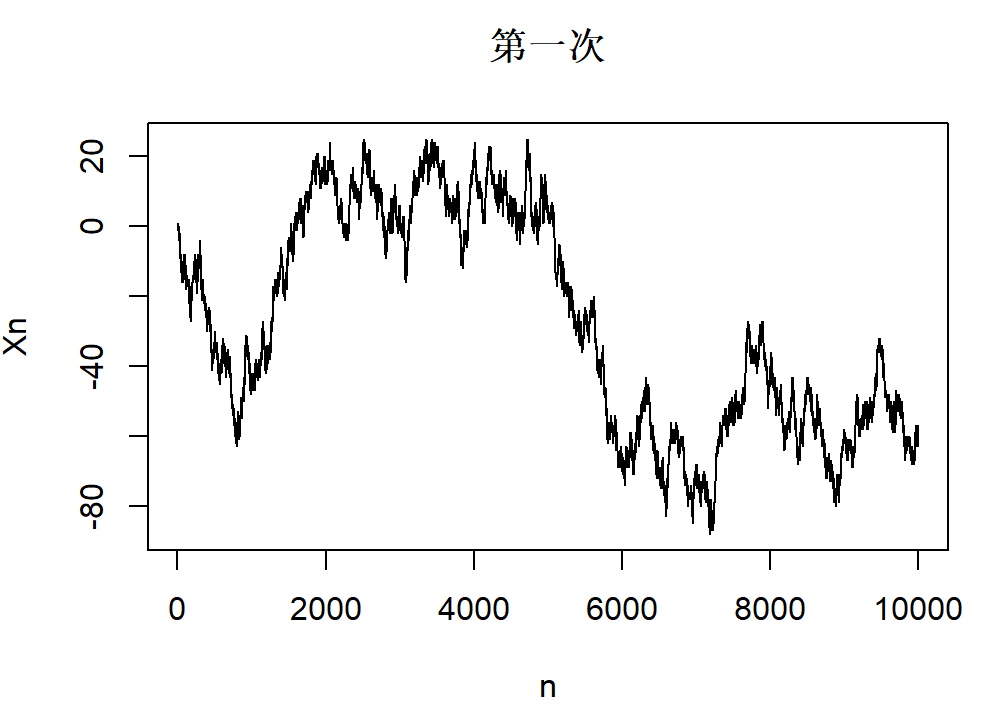
\includegraphics[scale=0.6]{random1.png}
\end{minipage}
\\
\begin{minipage}{0.5\textwidth}
    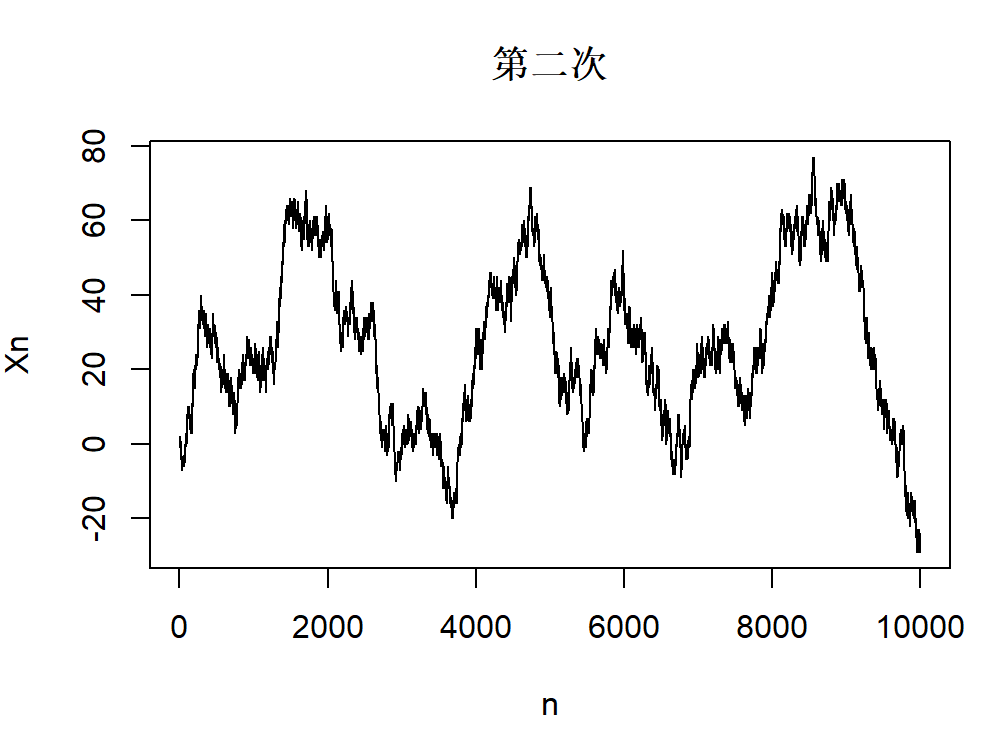
\includegraphics[scale=0.6]{random2.png}
\end{minipage}
\\
\begin{minipage}{0.5\textwidth}
    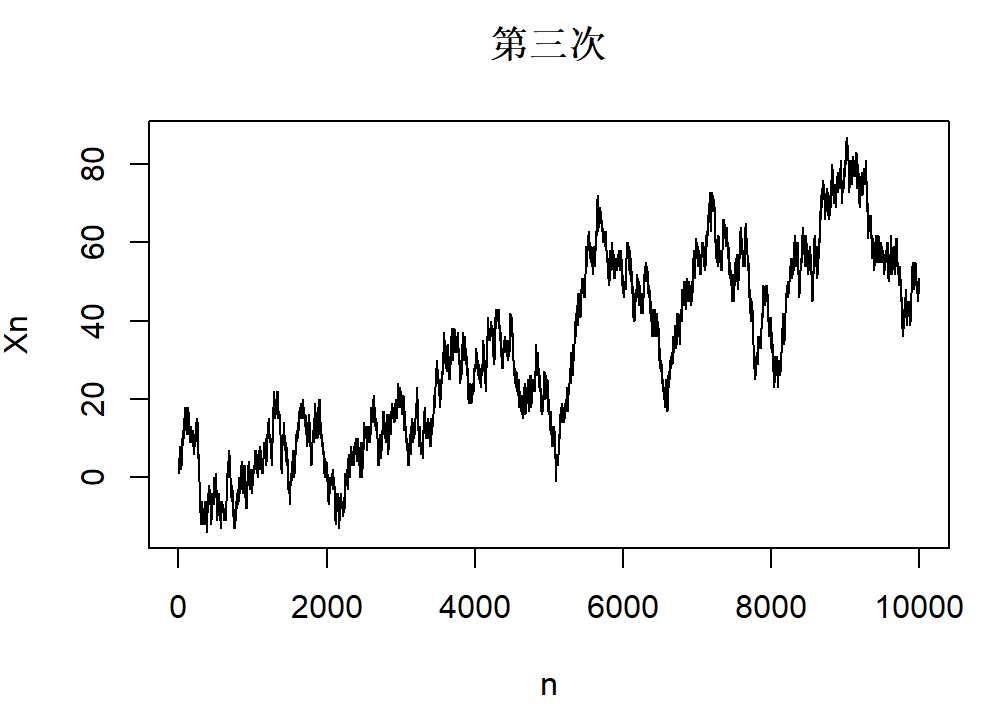
\includegraphics[scale=0.6]{random3.png}
\end{minipage}
\\
\begin{minipage}{0.5\textwidth}
    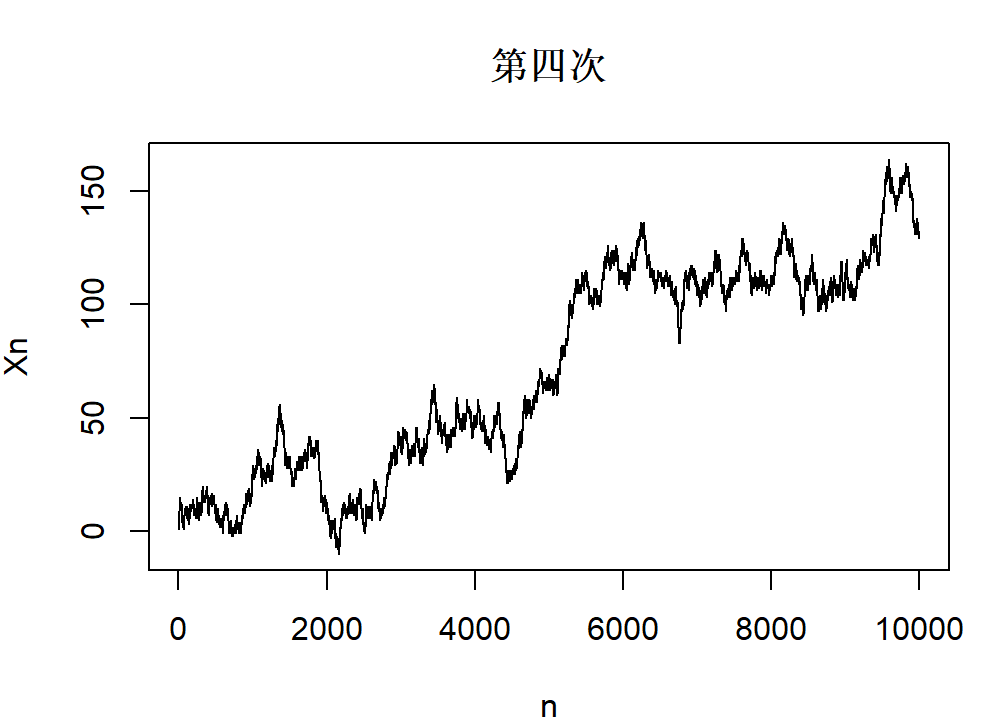
\includegraphics[scale=0.6]{random4.png}
\end{minipage}
\\
\begin{minipage}{0.5\textwidth}
    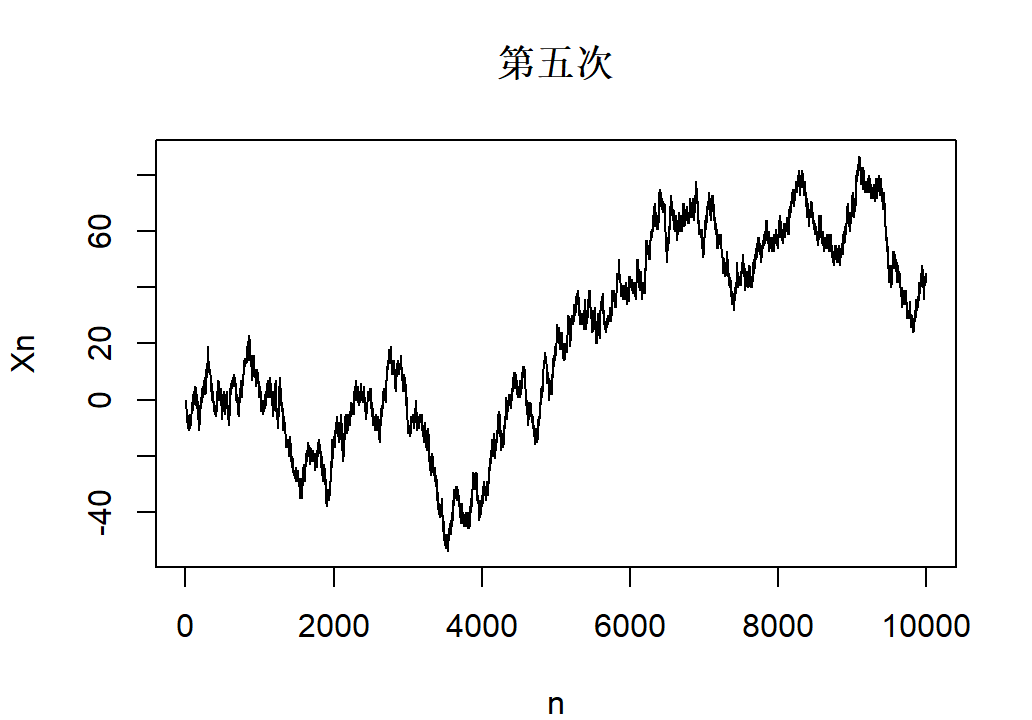
\includegraphics[scale=0.6]{random5.png}
\end{minipage}
\\
可以看出,随机序列整体呈现出非常随机的情况,并没有明显的集中趋势,并且某种程度上$n$越大,$X_{n}$偏离原点的趋势越明显.
\\同时,不同模拟之间图形呈现出显著的区别,有的正偏有的负偏,有的(如第四次)甚至偏移出非常远.
\\由于$E(X_{n})$,图形正偏和负偏自然是都有可能的,但因为$Var(X_{n})$与$n$成正比,随机徘徊位置和原点的平均偏差近似与$\sqrt{n}$成正比,因此产生出$n$越大越不可预测的结果.
\\由于$Var(X_{n})=\frac{n}{4}$,可以计算出$X_{10000}$的标准差为$50$,所以徘徊10000个时间周期后距离原点的距离基本在几十的数量级,较少数(如上面第四次)会偏差超过一百.
\end{CJK}
\end{document}